\chapter{陆地生态系统碳循环及其模型和数据}
\label{chap:model}
% - 章节意义:...是...的重点/前提,...有重大意义。
% - 本章内容:本章首先分析/阐述...,进一步...;接着探讨...;最后讨论...。针对框架构建的关键问题,分析现有框架设计的方法及其存在问题,提出了本文的重点内容。

\section{陆地生态系统碳循环}
% 介绍主要过程:光合、呼吸等
% 及影响因素
地球系统碳循环是指碳在岩石圈、水圈、大气圈和生物圈之间,以各种形式相互转换和迁移的过程。碳元素主要分布于陆地生态系统、海洋、大气和化石燃料四个碳库,其中陆地生态系统中的碳库是含量最小的碳库,但由于其是人类活动聚集的场所,所以又是最为活跃的碳库。它主要由植物光和器官碳库、植物支持器官碳库、凋落物碳库和土壤有机物碳库四部分组成,如图~\ref{fig:land-carbon-cycling-structure}所示,植物通过光合作用将大气中的$CO_2$转换为碳水化合物,再通过自养呼吸、分配光合作用产物和死亡凋落过程把碳输送到大气、植物支持器官碳库和凋落物碳库;植物支持器官通过自养呼吸和死亡凋落把有机碳分别输送到大气和凋落物碳库;凋落物碳库通过异样呼吸和分解作用分别把碳输送到大气和土壤有机物碳库中;土壤有机物碳库最后通过异样呼吸把碳输送回大气碳库中。因此,碳在陆地生态系统中的转移路径为:大气——植物光合器官——植物支持器官——凋落物——土壤——大气,形成了一个首尾相连的闭环,因此,可以把陆地生态系统中碳的转移看成一个循环过程。

\begin{figure}[!htbp]
    \centering
    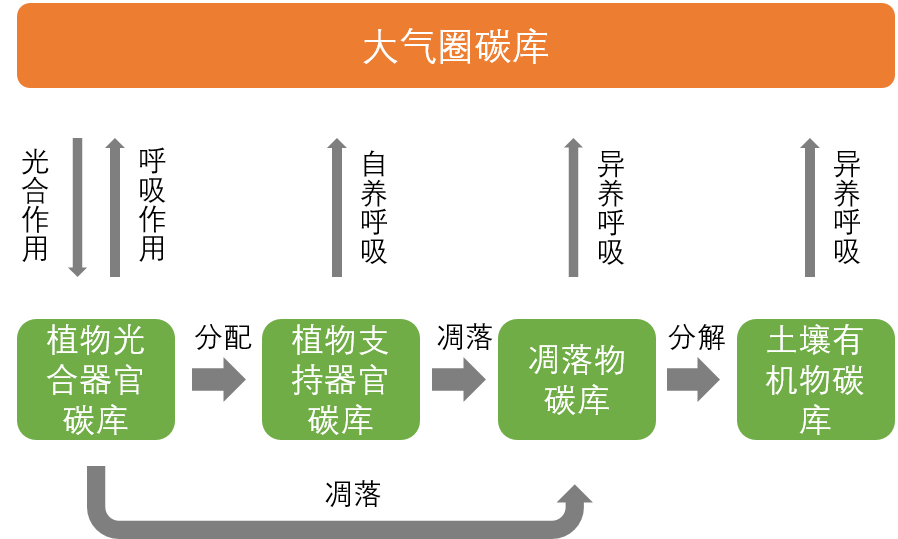
\includegraphics[width=0.9\textwidth]{land-carbon-cycling-structure}
    \caption{陆地生态系统碳循环基本过程}
    \label{fig:land-carbon-cycling-structure}
\end{figure}

\section{陆地生态系统碳循环模型}
% 介绍基本结构、特点、分类
\label{sec:model}
\subsection{陆地生态系统碳循环模型及其分类}
陆地生态系统碳循环中碳主要在植被——大气——土壤碳库之间转移,模型一般包括植物的光合作用、自养呼吸和异氧呼吸以及土壤的呼吸作用这四个过程,影响这些过程的因素有大气CO2浓度、辐射、气温、土壤湿度、叶片中的叶绿素含量,所以许多模型耦合了水循环过程和氮循环过程。陆地生态系统碳循环模型通过生物生产力来描述碳通量的变化,这些指标主要有总初级生产力(Gross Ecosystem Production,GPP)、净第一性生产力(Net Primary production,NPP)、净生态系统生产力(Net Ecosystem Production,NEP),他们之间的关系如公式~\ref{eq:NPP}和~\ref{eq:NEP}所示,式中,$R_A$表示自养呼吸,$R_H$表示异氧呼吸。

\begin{align}
    & NPP = GPP-R_A
    \label{eq:NPP} \\
    & NEP = \left(GPP-R_A\right)-R_H = NPP-R_H
    \label{eq:NEP}
\end{align}

除了这些指标外,模型计算过程中一般还包括有生物量(Biomass)、蒸散发(Evapotranspiration,ET)、径流(Runoff)、叶面积指数(LAI)等指标。

\begin{figure}[!htbp]
    \centering
    
\includegraphics[width=0.9\textwidth]{carbon-model-class}
    \caption{碳循环模型分类}
    \label{fig:carbon-model-class}
\end{figure}

陆地生态系统碳循环模型从机理上可分为统计模型、生态过程模型和遥感、过程耦合模型,如图~\ref{fig:carbon-model-class}所示。
统计模型可分为气候统计模型和遥感统计模型。其中气候统计模型主要通过在温度、降水等气候因子与植被净初级生产力(Net Primary Productivity,NPP)的实测数据之间建立回归方程,代表性的有Miami模型(曼阿密模型)~\cite{lieth1975modeling}、Chikugo模型(筑后模型)~\cite{seino1985agroclimatic}和Thornth-waite Memorial模型(桑斯维特纪念模型)~\cite{hai2012change};
遥感统计模型是基于遥感光谱指数建立的模型。由于总初级生产力(GPP)与截留光合有效辐射量和辐射的光合利用效率(LUE)成正比,而截留光合有效辐射与总光合有效辐射(PAR)和光合有效辐射截留率(FPAR)成正比。其中PAR可以通过气候学方法计算得到,FPAR可以通过遥感方法得到,因此,GPP可以表达为公式~\ref{eq:GPP},NPP可以表达为公式~\ref{eq:NPP}

\begin{align}
    &GPP(FPAR, PAR) = FPAR \cdot PAR \cdot LUE \cdot f(T, W, CO_2)
    \label{eq:GPP}  \\
    &NPP = GPP - R_A
    \label{eq:NPP}
\end{align}

式中,$f(T, W, CO_2)$表示温度T、土壤湿度W和大气中$CO_2$浓度对辐射的诗集光合利用效率的影响;$R_A$表示自养呼吸;代表性的模型有CASA、GLO-PEM、TURC、SIB2等
% 遥感统计模型主要通过遥感光谱指数(如NDVI)与植被净初级生产力、生物量等数据间的相关关系进行统计回归。
统计模型简单直观,具有较强的区域适用性,但其完全依赖于地面观测数据,对于不同的区域,模型不具备普适性和推广性。同时统计模型没有考虑陆地生态系统碳循环过程的内部机理,无法揭示生态系统与环境间的相互影响关系,不能用于对未来的预测研究~\cite{袁文平2014陆地生态系统植被生产力遥感模型研究进展}~\cite{谢馨瑶2018大尺度森林碳循环过程模拟模型综述}。

生态过程模型按照是否考虑实际环境对植被功能类型、组成和结构的影响分为基于动态植被类型的模型和基于静态植被类型的模型~\cite{王绍刚2008森林碳循环模型方法研究进展}~\cite{王萍2009基于}~\cite{毛留喜2006陆地生态系统碳循环模型研究概述},按照涉及到的机理类型分为地球化学过程模型、陆面物理过程模型和生物过程模型~\cite{谢馨瑶2018大尺度森林碳循环过程模拟模型综述}。过程模型由于其综合考虑了碳循环过程的动力学特征,结合了气候、土壤和植被生理生态参数,以及陆地生态系统与大气、海洋之间的相互作用,模拟结果相对来说更加准确,逐渐占据了主导地位。图~\ref{fig:DGVMs-structure}是生态过程模型的典型结构,其中冠层物理主要包括辐射传输、能量平衡、水平衡和气溶胶动力等过程,冠层生理主要用于计算光合作用和气孔导度,土壤物理包括能量平衡、水平衡和土壤温度等过程,自养呼吸主要指植被的维持呼吸和生长呼吸,异氧呼吸则指土壤呼吸和枯枝层分解,植被生理主要包括同化物分配和组织流转等过程,营养循环主要指碳、氮循环,植被竞争包括光竞争、水竞争和空间竞争,干扰过程主要涉及火灾、采伐( 或收割) 、林隙、热胁迫、干旱胁迫、背景胁迫( 如接近植被生命年限,死亡不可避免) 等,萌生过程主要指植被幼苗或种子在自然环境下的成活或萌发过程。生态过程模型的输入数据一般包括气象数据、CO2浓度数据、土壤质地数据、高程数据和植被功能类型数据等。

生态过程模型普遍采用植被功能类型(PFT)作为植被基本处理单元,通常将PFT划分为林地(覆盖热带、温带、寒带,常绿、落叶、针叶和阔叶等)、灌木(常绿和落叶等)、草地($C_3$、$C_4$等)、农田(水稻、玉米、温带谷物、大豆、热带根系作物、太阳花、花生、油菜等)等类型。每种植被功能类型对应有许多植被生理生态参数,如气孔导度、光合途径、叶片厚度等。

\begin{figure}[!htbp]
    \centering
    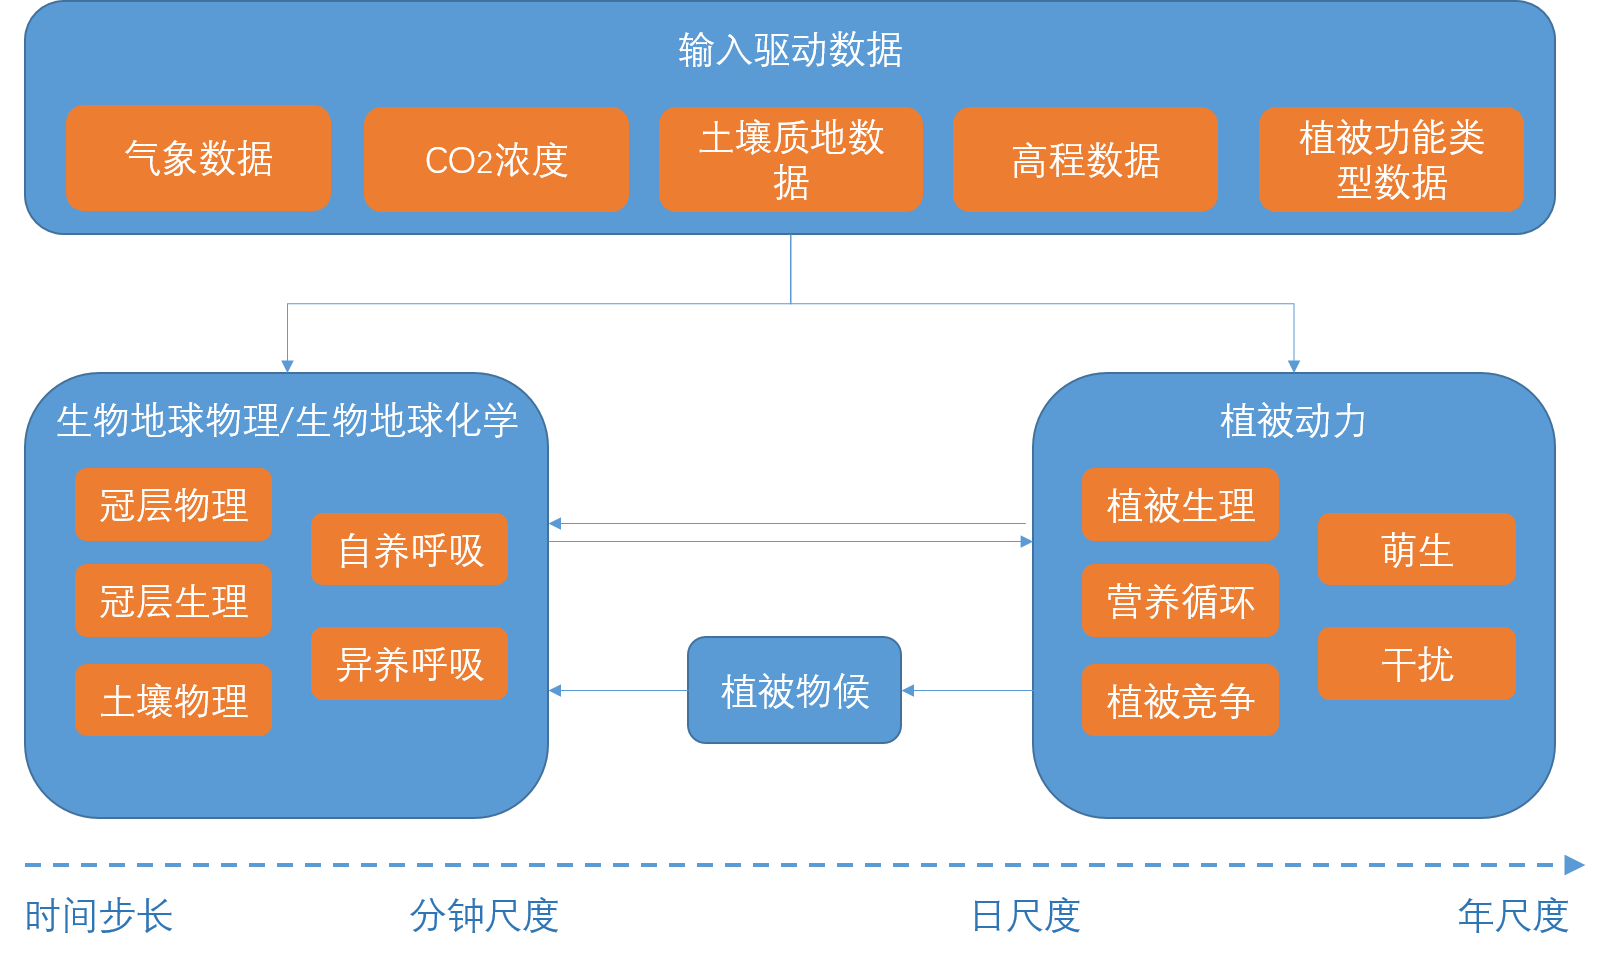
\includegraphics[width=0.9\textwidth]{DGVMs-structure}
    \caption{生态过程模型的典型结构}
    \label{fig:DGVMs-structure}
\end{figure}

遥感、过程耦合模型通过将遥感观测数据(如叶面积指数LAI)同化到模型之中,来提高模型模拟的精度(张延龙,2015),他融合了遥感统计模型和生态过程模型的优点,可以反映区域和全球尺度的NPP空间分布和变化~\cite{朱文泉2005陆地植被净初级生产力计算模型研究进展}。但由于遥感、过程耦合模型难度过大,在应用时不太方便。

综合分析三类模型的优缺点后,本文选取了IBIS、Biome-BGC、LPJ三个具有代表性的生态过程模型,在全球尺度上进行模拟和对比分析。

\subsection{IBIS, Biome-BGC, LPJ模型简介}
\subsubsection{IBIS模型}
% 起源、原理、结构、适用条件、输入数据、运行模式
IBIS全称为集成生物圈模拟器(Integrated BIosphere Simulator),由美国威斯康星——麦迪逊大学Foley等~\cite{foley1996integrated}提出,随后,Kucharik等~\cite{kucharik2000testing}于2000年对其进行了改进,现在最新版本是IBIS 2.6。模型包括地表模块、土壤地球生物化学模块、植被物候模块和植被动态模块5个模块,属于动态植被类型模型。IBIS模型综合考虑了地球化学过程、地球物理过程和植被动态过程,能够耦合大气环流模式,在时间上适用于跨度从秒到数百年的碳循环过程,在空间上适用的尺度包括斑块、景观、区域和全球。

IBIS模型的输入数据包括日分辨率的气象数据(平均温度、最大温度、最小温度、相对湿度、风速和云量)、土壤质地数据(沙粒含量、黏粒含量和粉粒含量)、植被功能类型(PFT)、网格点的经纬度。IBIS模型将植被功能类型分为12种,其中林地分为热带常绿阔叶林、热带干旱落叶阔叶林、温带常绿阔叶林、温带常绿针叶林、温带阔叶林、北方常绿针叶林、北方干旱落叶阔叶林、北方冷落叶针叶林,灌木和草地分为常绿灌木、冷落叶灌木、C3草本植物、C4草本植物,其他详细参数见Foley等~\cite{foley1996integrated},Kucharik等~\cite{kucharik2000testing}

\subsubsection{Biome-BGC模型}
Biome-BGC~\cite{thornton1998regional}~\cite{kimball1997simulating}~\cite{white2000parameterization}模型由美国蒙拿大大学森林学院陆地动态数值模拟团队(Numerical Terradynamic Simulation Group,NTSG)基于FOREST-BGC模型改进而来,广泛应用于模拟植被、凋落物、土壤中的碳、氮、水等物质的循环过程~\ref{Thornton2001Modeling}。模型使用静态植被类型,属于生物地球化学循环模型,包括的生理生态过程有光合作用、蒸散发、生态系统呼吸、分解、光合产物的分配以及植物的死亡,基本原理是物质和能量守恒定律,即进入生态系统中的物质和能量,等于离开生态系统的与生态系统中累积的之和。模型的植被功能类型被分为7类:落叶阔叶林、常绿阔叶林、常绿针叶林、灌木林、落叶针叶林、C3草本植物和C4草本植物,每种植被功能类型对应一套生理生态参数。该模型在空间上适用于区域尺度和全球尺度。

Biome-BGC模型的运行分为两阶段:spin-up阶段是获取模拟的初始状态,第二步是使用第一阶段的结果参数正式运行模拟程序,。初始状态的获取有两种方法,一是直接输入长期定点观测的参数值,二是运行模型自带的spin-up程序。在spin-up过程中,将模拟起点时的碳氮存量设为极低的值(叶片的碳存量为0.001$kg C/m^2$,其他库的碳氮存量均为0),反复模拟数千年,直到连续两年土壤碳差值小于0.005$kg C/m^2$,或达到设定的最大迭代年数为止,这时认为系统达到稳定状态~\cite{thornton2005ecosystem}~\cite{pietsch2005bgc}。


\subsubsection{LPJ模型}
% 11种作物功能类型
LPJ(Lund-potsdam-Jena Model,LPJ)~\cite{sitch2003evaluation}模型建立在Biome3模型的基础上,包括的植被生理过程包括光合作用、呼吸作用、植被冠层能量交换、土壤水平衡等。LPJ模型适用于大尺度、中尺度以及全球尺度范围内的碳循环模拟。LPJ模型的时间步长是1月,Venevsky~\ref{venevsky2007sever}对运行时间步长进行了修改,时间步长变成了1天。为了和IBIS模型与Biome-BGC模型的时间分辨率一致,本文应用的是Venevsky的LPJ-Daily。如无特殊说明,本文后面所说的LPJ均指LPJ-Daily。LPJ模型的植被功能类型分为10种,包括热带常绿阔叶林、热带雨绿阔叶林、温带常绿针叶林、温带常绿阔叶林、温带夏绿针叶林、北方常绿针叶林、北方夏绿针叶林、北方夏绿阔叶林、C3草本植物和C4草本植物。LPJ模型的运行也分为两个阶段:spin-up阶段假设没有植被(全为裸土地)和生物量,进行1000年积分直到植被覆盖和土壤碳达到平衡态;常规运行阶段使用spin-up阶段运行出的平衡态作为初始值进行模拟。与Biome-BGC不同的是,LPJ模型在内部将两个阶段直接串联在一起,不用分两步运行。


\section{陆地生态系统碳循环相关数据}
~\label{sec:model-data}
% 缺图:a陆面掩膜;b PFT;c DEM
% CO2 1982-2014 时间序列图
% FLUXNET 站点图(按PFT分类)/按年份分类
% 缺表:三个模型需要的数据对比表
本文所选的三个模型均以网格点为基本模拟单位,针对全球范围内的区域,本文使用$0.5^{\circ} \times 0.5^{\circ}$的经纬网划分格点,并筛选去除海洋和裸土地的格点,最终在全球范围内共有40595个格点。

如前文所分析,生态过程模型一般都需要气象数据集、土壤数据集和植被功能类型数据集,而在进行对比时,要确保使用相同的通用数据集。而由于不同模型对这些数据在时空分辨率、植被类型等方面的要求不同,因此,本文采用相同的数据域,针对每个模型的特殊要求,对原始数据进行数据处理。

\subsection{气象数据集}
本文采用MERRA 2(Modern Era Retrospective-analysis for Research and Applications 2)气象数据集,MERRA是NASA为卫星提供的在大气再分析资料,致力于天气和气候时间尺度与水循环相关研究,具有较高的空间分辨率和较完整的时间序列范围,气象要素包括平均温、最高温、最低温、相对湿度、降水量、风速和云量。本文的数据时间范围从1982年到2013年共32年,以日为时间分辨率。数据原始空间分辨率为$0.625^{\circ} \times 0.5^{\circ}$,对其进行重采样转换为$0.5^{\circ} \times 0.5^{\circ}$,以符合全球离散网格点的空间分布。

\subsection{土壤数据集}
主要包括土壤的颗粒组成成分,即沙粒含量、黏粒含量、粉粒含量、土壤深度,由中山大学土壤——大气相互作用研究组开发~\ref{shangguan2014global}。数据的空间分辨率为$0.0085^{\circ} \times 0.0107^{\circ}$,对其进行重采样转换为$0.5^{\circ} \times 0.5^{\circ}$。数据详情参考 \href{http://globalchange.bnu.edu.cn/research/soilw}{http://globalchange.bnu.edu.cn/research/soilw}

\subsection{植被功能类型数据集}
% 植被功能类型使用
生态过程模型普遍采用植被功能类型作为植被基本处理单元,本文所选的三个模型也是如此。由于这三个模型内部对植被功能类型的划分不同,因此对原始数据进行类型映射,如表~\ref{tab:IBIS-PFT-map}, ~\ref{tab:Biome-BGC-PFT-map}, ~\ref{tab:LPJ-PFT-map}所示,分别为三个模型的植被功能类型映射表。

\begin{table}[!htbp]
    \centering
    \caption{IBIS模型植被功能类型映射表}
    \label{tab:IBIB-PFT-map}
    \begin{threeparttable}
        \begin{tabular}{lcccccc}
            \Xhline{1.5pt}
            \multirow{2}{*}{\textbf{植被功能类型}} & \multicolumn{3}{c}{\textbf{生物量转换时间}} & \multicolumn{2}{c}{\textbf{碳分配系数}} & \multirow{2}{*}{\textbf{比叶面积}} \\ 
            \cline{2-4} \cline{5-6}
            & \textbf{叶} & \textbf{根} & \textbf{干} & \textbf{叶} & \textbf{根} &  \\ 
            \Xhline{1.5pt}
            \Xhline{1.5pt}
        \end{tabular}
        \begin{tablenotes}
            \footnotesize
            \item[]数据来源于Foley等~\cite{foley1996integrated}
        \end{tablenotes}
    \end{threeparttable}
\end{table}

\begin{table}[!htbp]
    \centering
    \caption{Biome-BGC模型植被功能类型映射表}
    \label{tab:Biome-BGC-PFT-map}
    \begin{threeparttable}
        \begin{tabular}{lcccccc}
            \Xhline{1.5pt} 
            \multirow{2}{*}{\textbf{植被功能类型}} & \multicolumn{3}{c}{\textbf{生物量转换时间}} & \multicolumn{2}{c}{\textbf{碳分配系数}} & \multirow{2}{*}{\textbf{比叶面积}} \\ 
            \cline{2-4} \cline{5-6}
            & \textbf{叶} & \textbf{根} & \textbf{干} & \textbf{叶} & \textbf{根} &  \\ 
            \Xhline{1.5pt}
            \Xhline{1.5pt}
        \end{tabular}
        \begin{tablenotes}
            \footnotesize
            \item[]数据来源于Foley等~\cite{foley1996integrated}
        \end{tablenotes}
    \end{threeparttable}
\end{table}

\begin{table}[!htbp]
    \centering
    \caption{LPJ模型植被功能类型映射表}
    \label{tab:LPJ-PFT-map}
    \begin{threeparttable}
        \begin{tabular}{lcccccc}
            \Xhline{1.5pt} 
            \multirow{2}{*}{\textbf{植被功能类型}} & \multicolumn{3}{c}{\textbf{生物量转换时间}} & \multicolumn{2}{c}{\textbf{碳分配系数}} & \multirow{2}{*}{\textbf{比叶面积}} \\ 
            \cline{2-4} \cline{5-6}
            & \textbf{叶} & \textbf{根} & \textbf{干} & \textbf{叶} & \textbf{根} &  \\ 
            \Xhline{1.5pt}
            \Xhline{1.5pt}
        \end{tabular}
        \begin{tablenotes}
            \footnotesize
            \item[]数据来源于Foley等~\cite{foley1996integrated}
        \end{tablenotes}
    \end{threeparttable}
\end{table}

\begin{figure}[!htbp]
    \centering
    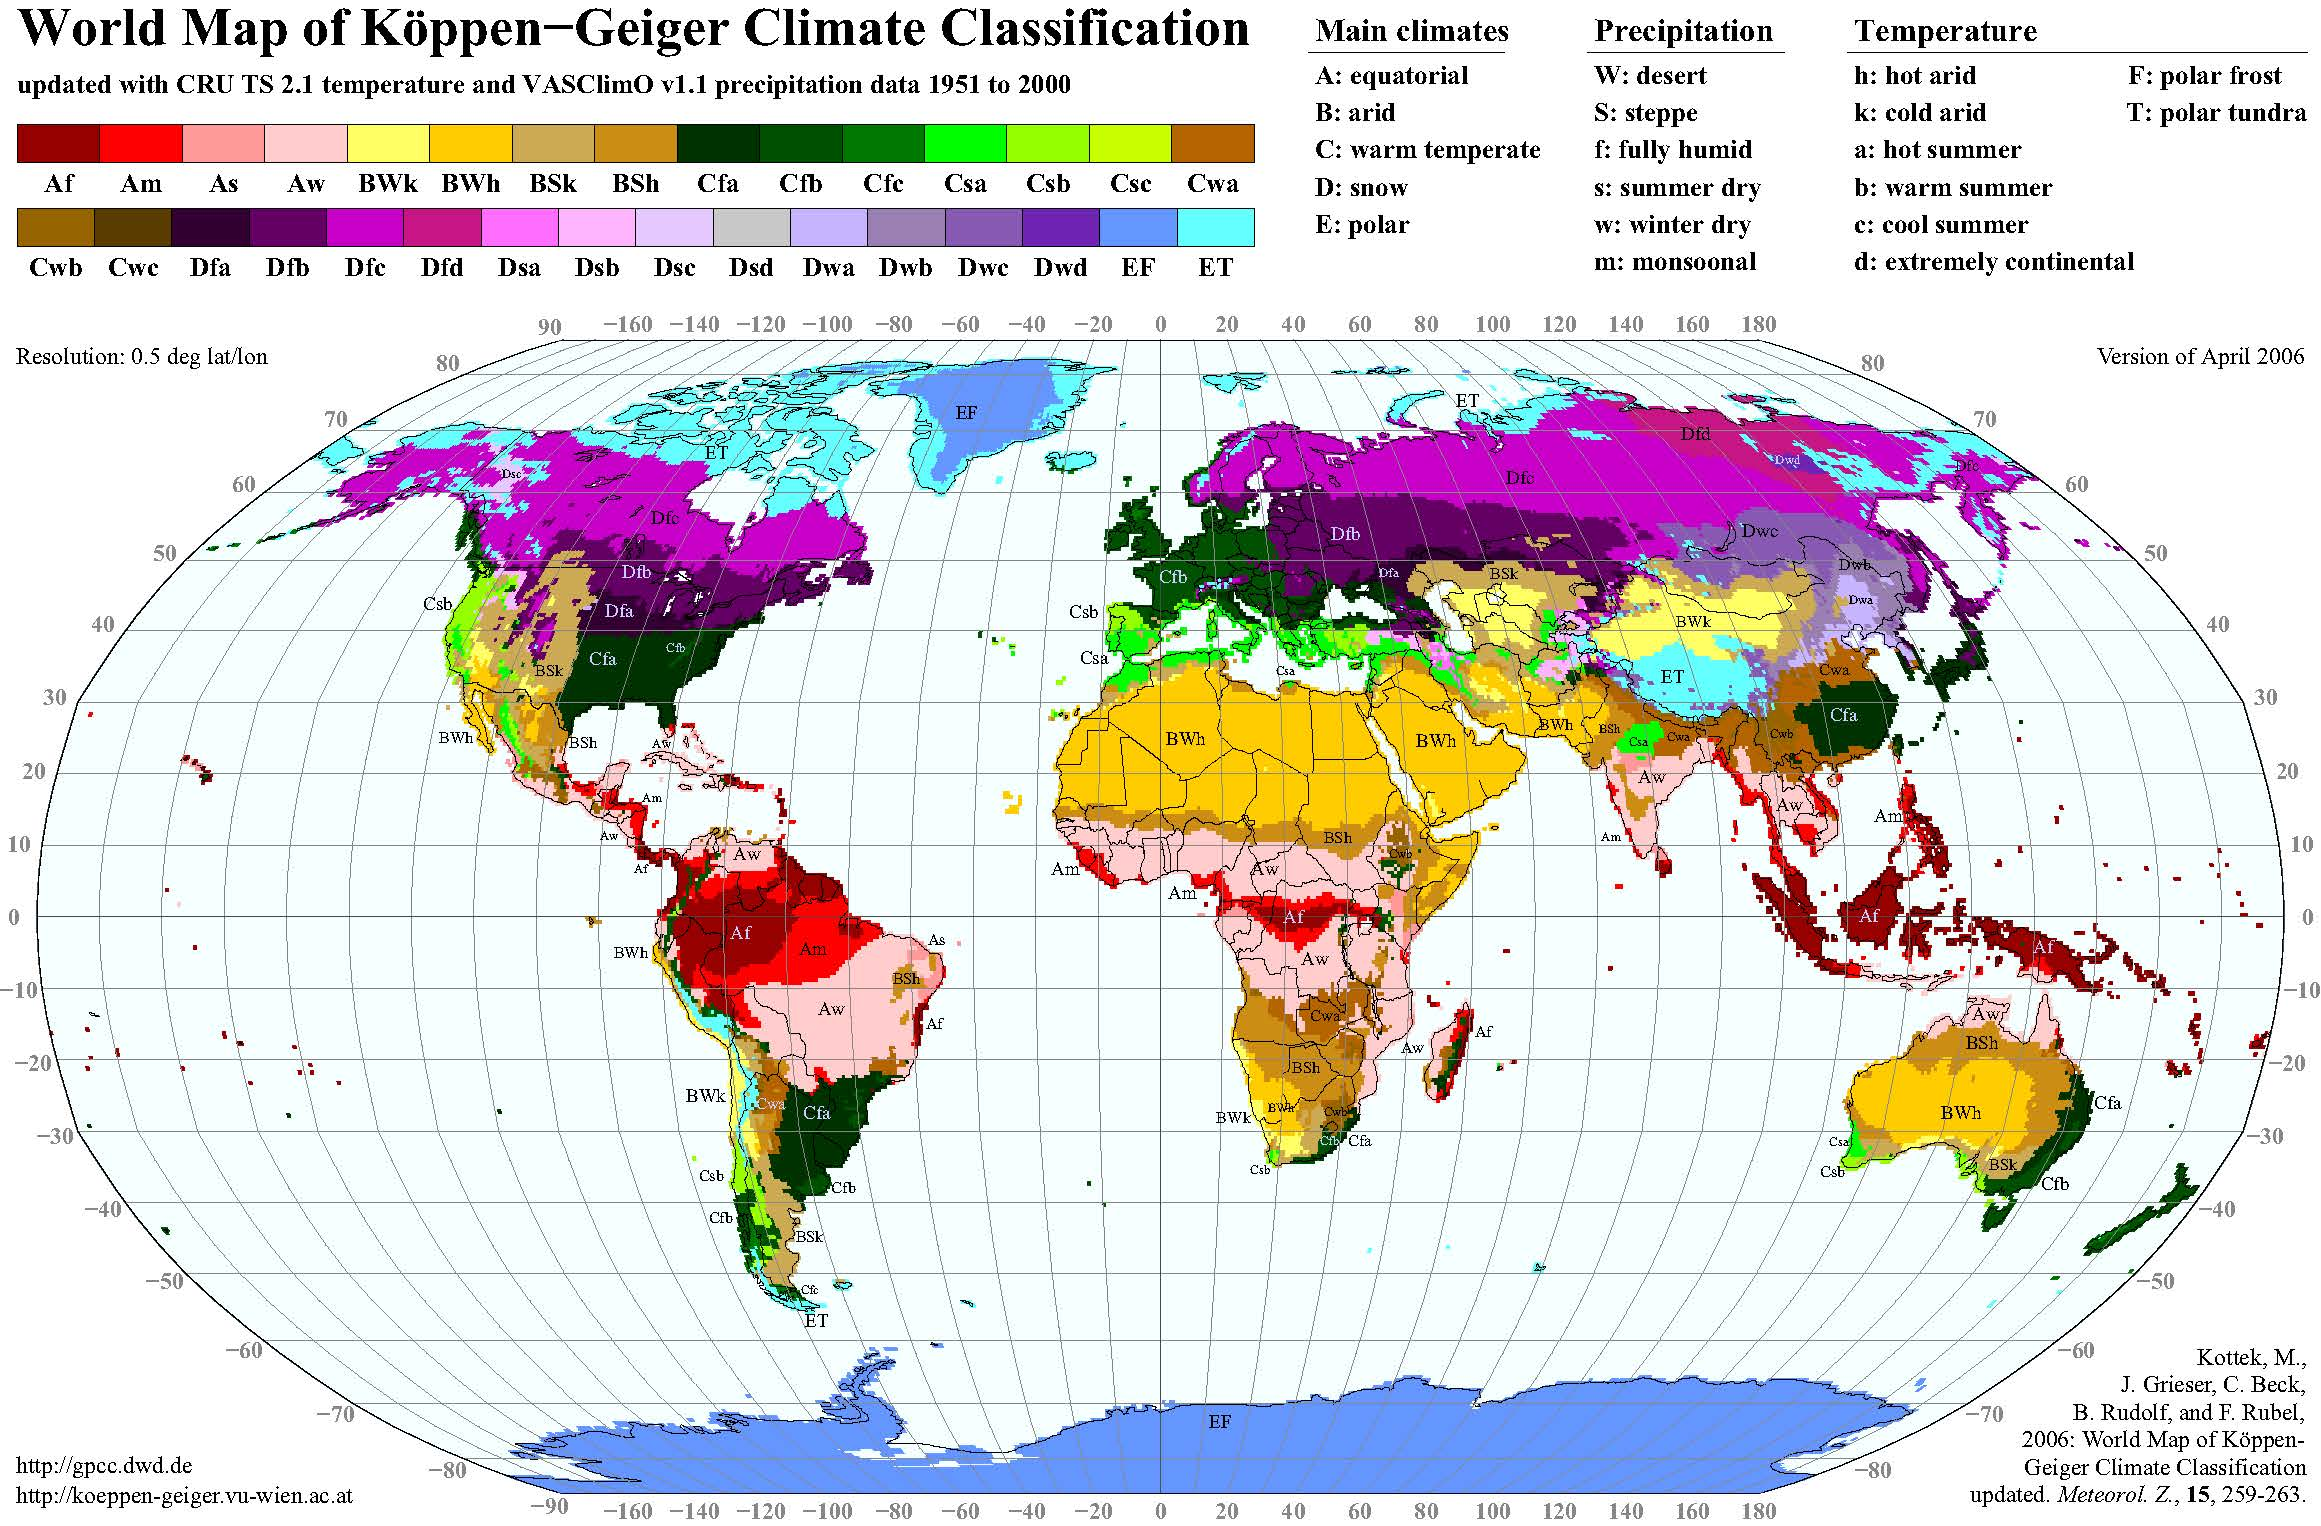
\includegraphics[width=0.9\textwidth]{PFT}
    \caption{植被功能类型图}
    \label{fig:PFT}
\end{figure}

\subsection{通量观测数据集}
% 举例的站点表
全球通量观测网络(FLUXNET)是一个以全球广泛分布的通量塔为基础的全球通量观测网络。通量观测站点遍布世界主要国家,在北美、欧洲、亚洲、非洲都有它的区域网络存在(如亚洲通量网AsiaFlux、美洲通量网AmeriFlux、中国通量网ChinaFlux)。到如今为止,累计有800多个活跃和历史的通量测定站点,分布在全球大部分气候空间和代表性生物群系中。覆盖的植被功能类型包括热带森林、温带针叶和阔叶森林、寒带森林、农田、草原、灌木丛、苔原和湿地。它在全球范围内连续测量大气状态变量,如温度、湿度、风速、降雨量、大气二氧化碳、植被生产力、生物量等。本文使用的是La Thuile数据集,包括站点每天的温度、降水、光合有效辐射比例(FPAR)、GPP、NEP,共计有231个通量观测站点,累计900余个站点$\cdot$年次数据,作为观测数据集与模型模拟的结果进行站点尺度上的对比。站点分布如图~\ref{fig:Thuile-site-POI}所示。

\begin{figure}[!htbp]
    \centering
    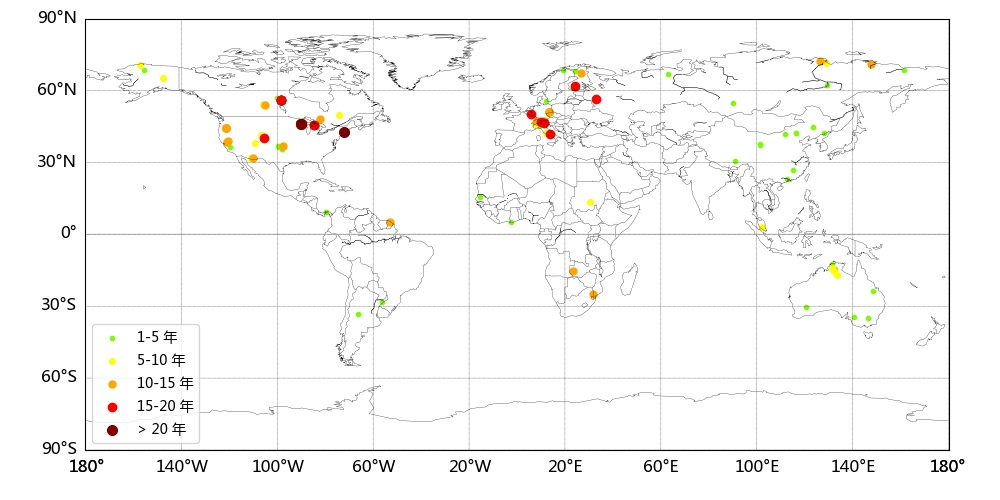
\includegraphics[width=1\textwidth]{sites-map}
    \caption{129个FLUXNET观测站点分布}
    \label{fig:sites-map}
\end{figure}

\begin{table}[!htbp]
    \centering
    \caption{站点植被功能类型统计表}
    \label{tab:site-PFT-stat}
    \begin{threeparttable}
        \begin{tabular}{c}
            \Xhline{1.5pt}
            \Xhline{1.5pt}
            \Xhline{1.5pt}
        \end{tabular}
    \end{threeparttable}
\end{table}

% 林地 草地 农田 湿地 灌木 草原 其他

% WET     Permanent Wetlands                  永久湿地
% CRO     Croplands                           农田
% MF      Mixed Forests                       混交林
% DBF     Deciduous Broadleaf Forests         落叶阔叶林          -
% EBF     Evergreen Broadleaf Forests         常绿阔叶林          -
% ENF     Evergreen Needleleaf Forests        常绿针叶林          -
% DNF     Deciduous Needleleaf Forests        落叶针叶林          -
% GRA     Grasslands                          草地                -
% WSA     Woody Savannas                      多树草原            -
% SAV     Savannas                            热带稀树草原
% OSH     Open Shrublands                     稀疏灌丛            -
% CSH     Closed Shrublands                   郁闭灌丛            -

\begin{table}[!htbp]
    \centering
    \caption{植被功能类型分类表}
    \label{tab:site-PFT-stat}
    \begin{threeparttable}
        \begin{tabular}{lllll}
            \Xhline{1.5pt}
            本文分类表 & FLUXNET & Biome-BGC & IBIS & LPJ \\
            \Xhline{1.5pt}
            \multirow{2}{*}{常绿针叶林} & \multirow{2}{*}{常绿针叶林} & \multirow{2}{*}{常绿针叶林} & 温带常绿针叶林 & \multirow{13}{*}{有分类体系,但是是根据气象数据和土壤数据计算出来,不做对应} \\
            &&& 北方常绿针叶林 & \\
            \multirow{3}{*}{落叶阔叶林} & \multirow{3}{*}{落叶阔叶林} & \multirow{3}{*}{落叶阔叶林} & 热带干旱落叶阔叶林 & \\
            &&& 北方干旱落叶阔叶林 & \\
            &&& 温带落叶阔叶林 & \\
            \multirow{2}{*}{常绿阔叶林} & \multirow{2}{*}{常绿阔叶林}& \multirow{2}{*}{常绿阔叶林} & 热带常绿阔叶林 & \\
            &&& 温带常绿阔叶林 & \\
            落叶针叶林 & 落叶针叶林 & 落叶针叶林 & 落叶针叶林 & \\
            \multirow{3}{*}{草本植物} & 草地 & \multirow{2}{*}{C3草本植物} & \multirow{2}{*}{C3草本植物} & \\
            & 多树草原 & & & \\
            & 热带稀树草原 & C4草本植物 & C4草本植物 & \\
            & 稀疏灌木 & \multirow{2}{*}{灌木} & 常绿灌木 & \\
            & 郁闭灌木 & & 冷落叶灌木 & \\
            \Xhline{1.5pt}
        \end{tabular}
    \end{threeparttable}
\end{table}



\subsection{MODIS GPP/NPP数据集}
MODIS MOD17 A3提供了时空连续的遥感GPP/NPP产品,MODIS/GPP产品以其他MODIS产品为基础计算而得,时间范围从2000年到2015年,时间分辨率为8天,空间分辨率为$0.0083^{\circ} \times 0.0083^{\circ}$,对其进行重采样转换为$0.5^{\circ} \times 0.5^{\circ}$。本文使用MODIS GPP/NPP 数据集作为全球尺度上的对比验证数据集,与三个模型模拟的结果进行对比分析。

\subsection{其他数据集}
模型还需要网格点的物理常量数据,包括有格点高程数据、短波反射率等。其中高程数据使用的是DEM数据

% \section{陆地生态系统碳循环模型对比方案分析和归纳}
% \subsection{基于实验协议的模型对比方案}
% % CMIP

% \subsection{可迁移、复用与重现的模型对比方案}
% % CORDEX
% % 基于虚拟机镜像/包管理器/docker

% \subsection{陆地生态系统碳循环模型对比方案总结}
% % 这一部分很重要,要明确的说明以上方案的不足之处
% % 引出我们的对比方案的优点和设计
% % 这是立题之本

% 传统的模型对比框架是以数据为基础,不考虑生产数据即模型模拟的过程。

% \section{本章小结}
% 本章首先从地球系统碳循环和陆地生态系统碳循环两部分分析了碳循环的过程;接着总结了陆地生态系统碳循环模型的基本结构和分类体系,并详细介绍了本文所对比的三个生态过程碳循环模型:IBIS、Biome-BGC和LPJ;最后针对这些模型所需要的数据做出了详细的介绍。